\section*{致谢}
感谢 Andre Walker-Loud 不断的鼓励以及对稿件的关键性阅读。
感谢 R. Harlander 与 T. Luu 对初稿改进的建议。
感谢与 R. Harlander、J. Kim、T. Luu、E. Mereghetti、C. Monahan、M. Rizik、
P. Stoffer 和 A. Walker-Loud 关于梯度流的多次讨论。
感谢劳伦斯伯克利国家实验室核理论组以及加州大学伯克利分校的接待。
本研究由德国研究联合会（DFG，grant 513989149）以及美国国家科学基金会
Grant No. PHY-2209185 资助。

\newpage
\section{补充材料}\label{SupplMat}

本文提出的方法至少在原则上适用于计算部分子分布函数的任意矩，
从而解决了格点上 twist-2 算符重正化这一长期存在的问题。
实际上，式~\eqref{eq:flowed_t2} 中带流 twist-2 算符强子矩阵元的
格点 QCD 计算受若干系统不确定度制约。

\subsection{有限体积效应}
在连续极限下，式~\eqref{eq:flowed_t2} 中带流 twist-2 算符的时空延展
由流时间半径 $\sqrt{8t}$ 决定，
强子矩阵元的有限体积效应可用有效场论方法计算~\cite{Detmold:2005pt}。
在有限格距 $a$ 处，有限体积限制了协变导数的数目，
从而限制了可模拟矩的阶数。算符 $\widehat{\rO}_n^{rs}(x,t)$
含 $n-1$ 个导数，规范链离开 $x$ 的最远距离为 $(n-1)a$。
现在考虑在时间长度为 $T$ 的格点上计算的 $\widehat{\rO}_n^{rs}(x,t)$
介子矩阵元一例。带流算符最大延展的合理估计约为 $\sim T/8$。
对当前最先进的格点 QCD 模拟，这意味着直到 $n \sim 10$
强子矩阵元的计算都不应受到阻碍。
对核子矩阵元，信噪比可能给出更强的约束，下文将予讨论。

\subsection{离散化误差}
当 $\sqrt{8t}$ 小于 $\simeq n a$ 时，$\llangle x^n \rrangle (t)$
的计算可预期存在可观的离散化误差；
对更大的 $\sqrt{8t}$ 值，没有理由预期出现不同于其他类似计算的离散化效应。
此外，格点 QCD 计算中常见做法是构造特定比值，
使部分潜在系统效应得以约减。

诸如式~\eqref{eq:Rn} 定义的 $R_n^h(t)$ 这类比值的典型用途，
是相对标准 twist-2 强子矩阵元大幅压低截断效应。
对非微扰改进 Wilson 费米子情形，
这一点也可由基于 Symanzik 有效理论方法的理论分析证实。
文献~\cite{Luscher:2013cpa} 已证明：除通常随理论非微扰 O($a$) 改进
被消除的 O($a$) 截断效应外，
仅存的附加截断效应为 O($am$)（$m$ 为夸克质量）\footnote{涉及带流场的格点关联函数原则上可能受短距离 O($a$) 截断效应影响，但在强子矩阵元计算中预计可忽略（参见文献~\cite{Kim:2021qae} 中这些短距离 O($a$) 截断效应可忽略的另一例子）。}。
这些截断效应只依赖可观测量的费米子内容，
因此在比值 $R_n^h(t)$ 中相消。
剩下的只是只受 O($a^2$) 效应影响的格点关联函数比值。

\subsection{微扰匹配}
匹配系数的微扰计算遵循标准策略
（参见 \cite{Manohar:2018aog,Mereghetti:2021nkt} 及其中文献）：
固定 $t$，把匹配方程~\eqref{eq:matching_eq} 圈积分的被积函数
对所有软标度展开。
式~\eqref{eq:matching_eq} 右端 $t=0$ 的单圈贡献为零，
因为展开导致 D 维中无标度即为零的积分。
在对规范耦合和带流费米子场重正化之后，左端 UV 有限。
由软标度展开产生、并以维数正规化调节的红外奇异性，
恰好与 $Z_n^{\MS}$ 的 UV 极点匹配。有限的匹配系数即此流程的结果。

相关费曼图绘于图~\ref{fig:fd}\footnote{费曼图用 FeynGame 绘制~\cite{Harlander:2020cyh}。}。
叉号表示 twist-2 算符插入，
单直线的单波浪线分别表示费米子与胶子传播子，
双直线表示费米子型 GF 微分算符的核。
空心圆表示 GF 顶点，其余为标准 QCD 顶点。
算符的费曼规则与非流情形相同，
与 GF 方程展开相关的其余费曼规则可参见例如
文献~\cite{Rizik:2020naq,Mereghetti:2021nkt}。

\begin{figure}[htbp]
  \centering
  
\includegraphics[width=0.11\textwidth]{images/vertex.pdf}
  \includegraphics[width=0.11\textwidth]{images/sail.pdf}
  \includegraphics[width=0.11\textwidth]{images/sail_1fk.pdf}
  \includegraphics[width=0.11\textwidth]{images/vertex_1fk.pdf}
  \includegraphics[width=0.11\textwidth]{images/vertex_2fk.pdf}
  \includegraphics[width=0.11\textwidth]{images/self_1fk.pdf}
  \includegraphics[width=0.11\textwidth]{images/self_2fk.pdf}
  \includegraphics[width=0.11\textwidth]{images/self_tad.pdf}
  \caption{式~\eqref{eq:matching_eq} 匹配系数 O($\gbar^2$) 计算的费曼图。
  带叉圆圈表示 twist-2 算符，空心圆表示 GF 顶点。
  双线表示 GF 微分算符的费米子型核。
  费米线与核线旁的箭头指示流时间增大的方向。}
  \label{fig:fd}
\end{figure}

计算的最终结果由式~\eqref{eq:matching_1l} 给出。
匹配系数满足一个重正化群（RG）方程；
利用``环化''矩阵元或式~\eqref{eq:ratio_n2} 中带流矩阵元之比
是重正化群不变量这一事实即可确定该方程。
RG 方程的解 $c_n^{\text{RG}}(t,\mu)$ 为
\be
c_n^{\text{RG}}(t,\mu) = c_n(\gbar(q))
\text{exp}\left\{-\int_{\gbar(\mu)}^{\gbar(q)}dx \frac{\gamma_n(x)}{\beta(x)}\right\}\,,
\label{eq:cn_resum}
\ee
其中 $\beta$ 是 beta 函数，$\gamma_n$ 是式~\eqref{eq:t2} 中 twist-2 算符的反常量纲。
匹配系数 $c_n(\gbar(q))$ 即式~\eqref{eq:cn_1l} 中取 $q=1/\sqrt{t}$ 的匹配系数。
我们把 $\beta(\gbar)$ 的微扰展开取到 $\gbar^5$ 阶~\cite{Jones:1974mm}，
把 $\gamma_n(\gbar)$ 取到 $\gbar^4$ 阶~\cite{Floratos:1977au,Gonzalez-Arroyo:1979guc,Curci:1980uw}，
并求出式~\eqref{eq:cn_resum} 中的次领头对数（NLL）表达式
$c_n^{\text{NLL}}(t,\mu)$。
\begin{figure}[htbp]
\centering
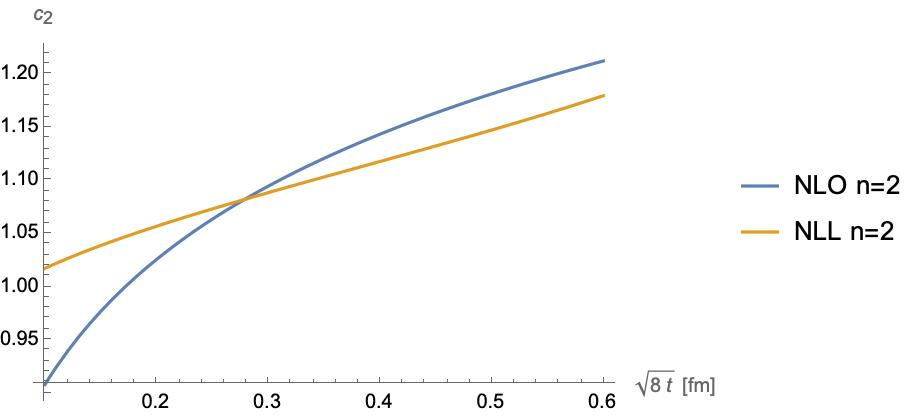
\includegraphics[width=7.5cm]{images/c2resum.jpg}
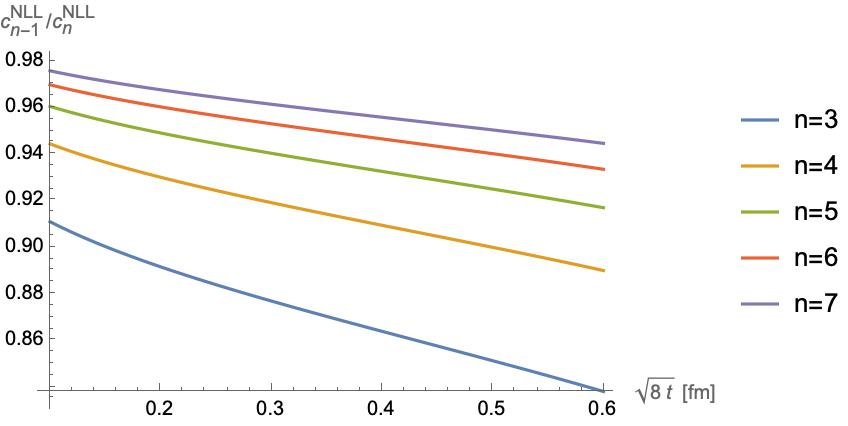
\includegraphics[width=7.5cm]{images/cnLLratio.jpg}
\caption{左图：$\mu=2$ GeV 处二阶矩匹配系数的流时间依赖，比较 NLO 结果与重求和结果。
右图：$\mu=2$ GeV 处比值 $c_{n-1}^{\text{NLL}}(\mu,t)/c_n^{\text{NLL}}(\mu,t)$ 的流时间依赖。}
\label{fig:running}
\end{figure}
取 $\mu=2$ GeV，二阶矩 $\llangle x \rrangle$ 的微扰修正
在流时间半径 $\sqrt{8t}=0.2-0.3$ fm 区域内介于 $6-9\%$ 之间。
图~\ref{fig:running} 左图展示二阶矩的匹配系数，
比较了 $\mu=2$ GeV 时式~\eqref{eq:matching_1l} 与式~\eqref{eq:cn_resum}
的重求和结果随 $\sqrt{8t}$ 的变化。
流时间半径的范围选在格距 $a=0.05-0.08$ fm 时不会出现大截断效应的区域。
我们观察到重求和保证耦合在 $t \rightarrow 0$ 极限下平滑趋于零。
在格点 QCD 模拟中，完成微扰匹配后，
残余流时间依赖可通过把数值数据向 $t \rightarrow 0$ 外推而去除。
对涉及带流可观测量的计算这是标准做法
（例如参见文献~\cite{Black:2023vju}）。

对更高阶矩，我们考虑式~\eqref{eq:Rn} 中的比值，
借助式~\eqref{eq:ratio_n2} 可用它计算 $\MSbar$ 方案中的矩。
再次固定重正化标度 $\mu=2$ GeV，
图~\ref{fig:running} 右图展示比值
$\frac{c_{n-1}^{\text{NLL}}(t,\mu,\gbar(\mu))}{c_n^{\text{NLL}}(t,\mu,\gbar(\mu))}$
随 $\sqrt{8t}$ 的变化（$n=3,\cdots, 7$）。我们看到微扰修正随 $n$ 增大而减小。
为初步估计 NLL 微扰匹配的预期不确定度，
我们在 $\sqrt{8t} = 2 (n-1) a$
（即距 twist-2 局域算符最远可能贡献两倍的距离）处
计算了高阶矩的微扰修正 $\delta_{\text{PT}}$。
估计取格距 $a=0.05$ fm——当前最先进格点 QCD 模拟可达到的格距。
结果列于表~\ref{tab:pert}。

\begin{table}[htbp]
  \centering
   \begin{tabular}{|c|c|c|}
   \hline
   $n$ & $\llangle x^{n-1} \rrangle$ & $\delta_{\text{PT}}$ \\ [0.5ex]
   \hline
   2 & $\llangle x \rrangle$     & $2\%$   \\
   3 & $\llangle x^{2} \rrangle$ & $11\%$  \\
   4 & $\llangle x^{3} \rrangle$ & $8\%$   \\
   5 & $\llangle x^{4} \rrangle$ & $7\%$   \\
   6 & $\llangle x^{5} \rrangle$ & $6\%$   \\
   7 & $\llangle x^{6} \rrangle$ & $6\%$   \\ [1ex]
   \hline
   \end{tabular}
   \caption{$\mu=2$ GeV、$\sqrt{8t} = 2(n-1) a$、$a=0.05$ fm 时 PDF 各阶矩的微扰修正。}
   \label{tab:pert}
  \end{table}

由此练习可以得出结论：至少在 NLL 微扰论水平，
比值 $R_n^h(t)$ 的流时间依赖非常小；
在晶格离散化效应应受控的 $\sqrt{8t}$ 区域内也是如此。
完成微扰匹配后，可以设想更高维算符会贡献于矩阵元的流时间依赖；
这实际上在所有局域带流算符矩阵元计算中都已被观察到。
通行做法是把匹配结果向 $t \rightarrow 0$ 外推；
外推通常非常平滑并能消除残余流时间依赖。
只有透彻的数值研究才能确认这些预期，
但可以设想使用比值 $R_n^h(t)$ 也有利于削弱更高维算符的贡献。
总之，选取重正化标度 $\mu=2$ GeV，
可以确定微扰修正很小、且流时间高阶贡献可平滑外推到零的
矩阵元比值。

\begin{thebibliography}{53}%
\makeatletter
\providecommand \@ifxundefined [1]{%
 \@ifx{#1\undefined}
}%
\providecommand \@ifnum [1]{%
 \ifnum #1\expandafter \@firstoftwo
 \else \expandafter \@secondoftwo
 \fi
}%
\providecommand \@ifx [1]{%
 \ifx #1\expandafter \@firstoftwo
 \else \expandafter \@secondoftwo
 \fi
}%
\providecommand \natexlab [1]{#1}%
\providecommand \enquote  [1]{``#1''}%
\providecommand \bibnamefont  [1]{#1}%
\providecommand \bibfnamefont [1]{#1}%
\providecommand \citenamefont [1]{#1}%
\providecommand \href@noop [0]{\@secondoftwo}%
\providecommand \href [0]{\begingroup \@sanitize@url \@href}%
\providecommand \@href[1]{\@@startlink{#1}\@@href}%
\providecommand \@@href[1]{\endgroup#1\@@endlink}%
\providecommand \@sanitize@url [0]{\catcode `\\12\catcode `\$12\catcode
  `\&12\catcode `\#12\catcode `\^12\catcode `\_12\catcode `\%12\relax}%
\providecommand \@@startlink[1]{}%
\providecommand \@@endlink[0]{}%
\providecommand \url  [0]{\begingroup\@sanitize@url \@url }%
\providecommand \@url [1]{\endgroup\@href {#1}{\urlprefix }}%
\providecommand \urlprefix  [0]{URL }%
\providecommand \Eprint [0]{\href }%
\providecommand \doibase [0]{https://doi.org/}%
\providecommand \selectlanguage [0]{\@gobble}%
\providecommand \bibinfo  [0]{\@secondoftwo}%
\providecommand \bibfield  [0]{\@secondoftwo}%
\providecommand \translation [1]{[#1]}%
\providecommand \BibitemOpen [0]{}%
\providecommand \bibitemStop [0]{}%
\providecommand \bibitemNoStop [0]{.\EOS\space}%
\providecommand \EOS [0]{\spacefactor3000\relax}%
\providecommand \BibitemShut  [1]{\csname bibitem#1\endcsname}%
\let\auto@bib@innerbib\@empty
%</preamble>
\bibitem [{\citenamefont {Collins}\ \emph {et~al.}(1989)\citenamefont
  {Collins}, \citenamefont {Soper},\ and\ \citenamefont
  {Sterman}}]{Collins:1989gx}%
  \BibitemOpen
  \bibfield  {author} {\bibinfo {author} {\bibfnamefont {J.~C.}\ \bibnamefont
  {Collins}}, \bibinfo {author} {\bibfnamefont {D.~E.}\ \bibnamefont {Soper}},\
  and\ \bibinfo {author} {\bibfnamefont {G.~F.}\ \bibnamefont {Sterman}},\
  }\bibfield  {title} {\bibinfo {title} {{Factorization of Hard Processes in
  QCD}},\ }\href {https://doi.org/10.1142/9789814503266_0001} {\bibfield
  {journal} {\bibinfo  {journal} {Adv. Ser. Direct. High Energy Phys.}\
  }\textbf {\bibinfo {volume} {5}},\ \bibinfo {pages} {1} (\bibinfo {year}
  {1989})},\ \Eprint {https://arxiv.org/abs/hep-ph/0409313}
  {arXiv:hep-ph/0409313} \BibitemShut {NoStop}%
\bibitem [{\citenamefont {Gribov}\ and\ \citenamefont
  {Lipatov}(1972)}]{Gribov:1972ri}%
  \BibitemOpen
  \bibfield  {author} {\bibinfo {author} {\bibfnamefont {V.~N.}\ \bibnamefont
  {Gribov}}\ and\ \bibinfo {author} {\bibfnamefont {L.~N.}\ \bibnamefont
  {Lipatov}},\ }\bibfield  {title} {\bibinfo {title} {{Deep inelastic e p
  scattering in perturbation theory}},\ }\href@noop {} {\bibfield  {journal}
  {\bibinfo  {journal} {Sov. J. Nucl. Phys.}\ }\textbf {\bibinfo {volume}
  {15}},\ \bibinfo {pages} {438} (\bibinfo {year} {1972})}\BibitemShut
  {NoStop}%
\bibitem [{\citenamefont {Lipatov}(1974)}]{Lipatov:1974qm}%
  \BibitemOpen
  \bibfield  {author} {\bibinfo {author} {\bibfnamefont {L.~N.}\ \bibnamefont
  {Lipatov}},\ }\bibfield  {title} {\bibinfo {title} {{The parton model and
  perturbation theory}},\ }\href@noop {} {\bibfield  {journal} {\bibinfo
  {journal} {Yad. Fiz.}\ }\textbf {\bibinfo {volume} {20}},\ \bibinfo {pages}
  {181} (\bibinfo {year} {1974})}\BibitemShut {NoStop}%
\bibitem [{\citenamefont {Dokshitzer}(1977)}]{Dokshitzer:1977sg}%
  \BibitemOpen
  \bibfield  {author} {\bibinfo {author} {\bibfnamefont {Y.~L.}\ \bibnamefont
  {Dokshitzer}},\ }\bibfield  {title} {\bibinfo {title} {{Calculation of the
  Structure Functions for Deep Inelastic Scattering and e+ e- Annihilation by
  Perturbation Theory in Quantum Chromodynamics.}},\ }\href@noop {} {\bibfield
  {journal} {\bibinfo  {journal} {Sov. Phys. JETP}\ }\textbf {\bibinfo {volume}
  {46}},\ \bibinfo {pages} {641} (\bibinfo {year} {1977})}\BibitemShut
  {NoStop}%
\bibitem [{\citenamefont {Altarelli}\ and\ \citenamefont
  {Parisi}(1977)}]{Altarelli:1977zs}%
  \BibitemOpen
  \bibfield  {author} {\bibinfo {author} {\bibfnamefont {G.}~\bibnamefont
  {Altarelli}}\ and\ \bibinfo {author} {\bibfnamefont {G.}~\bibnamefont
  {Parisi}},\ }\bibfield  {title} {\bibinfo {title} {{Asymptotic Freedom in
  Parton Language}},\ }\href {https://doi.org/10.1016/0550-3213(77)90384-4}
  {\bibfield  {journal} {\bibinfo  {journal} {Nucl. Phys. B}\ }\textbf
  {\bibinfo {volume} {126}},\ \bibinfo {pages} {298} (\bibinfo {year}
  {1977})}\BibitemShut {NoStop}%
\bibitem [{\citenamefont {Curci}\ \emph {et~al.}(1980)\citenamefont {Curci},
  \citenamefont {Furmanski},\ and\ \citenamefont {Petronzio}}]{Curci:1980uw}%
  \BibitemOpen
  \bibfield  {author} {\bibinfo {author} {\bibfnamefont {G.}~\bibnamefont
  {Curci}}, \bibinfo {author} {\bibfnamefont {W.}~\bibnamefont {Furmanski}},\
  and\ \bibinfo {author} {\bibfnamefont {R.}~\bibnamefont {Petronzio}},\
  }\bibfield  {title} {\bibinfo {title} {{Evolution of Parton Densities Beyond
  Leading Order: The Nonsinglet Case}},\ }\href
  {https://doi.org/10.1016/0550-3213(80)90003-6} {\bibfield  {journal}
  {\bibinfo  {journal} {Nucl. Phys. B}\ }\textbf {\bibinfo {volume} {175}},\
  \bibinfo {pages} {27} (\bibinfo {year} {1980})}\BibitemShut {NoStop}%
\bibitem [{\citenamefont {Collins}\ and\ \citenamefont
  {Soper}(1982)}]{Collins:1981uw}%
  \BibitemOpen
  \bibfield  {author} {\bibinfo {author} {\bibfnamefont {J.~C.}\ \bibnamefont
  {Collins}}\ and\ \bibinfo {author} {\bibfnamefont {D.~E.}\ \bibnamefont
  {Soper}},\ }\bibfield  {title} {\bibinfo {title} {{Parton Distribution and
  Decay Functions}},\ }\href {https://doi.org/10.1016/0550-3213(82)90021-9}
  {\bibfield  {journal} {\bibinfo  {journal} {Nucl. Phys. B}\ }\textbf
  {\bibinfo {volume} {194}},\ \bibinfo {pages} {445} (\bibinfo {year}
  {1982})}\BibitemShut {NoStop}%
\bibitem [{\citenamefont {Kronfeld}\ and\ \citenamefont
  {Photiadis}(1985)}]{Kronfeld:1984zv}%
  \BibitemOpen
  \bibfield  {author} {\bibinfo {author} {\bibfnamefont {A.~S.}\ \bibnamefont
  {Kronfeld}}\ and\ \bibinfo {author} {\bibfnamefont {D.~M.}\ \bibnamefont
  {Photiadis}},\ }\bibfield  {title} {\bibinfo {title} {{Phenomenology on the
  Lattice: Composite Operators in Lattice Gauge Theory}},\ }\href
  {https://doi.org/10.1103/PhysRevD.31.2939} {\bibfield  {journal} {\bibinfo
  {journal} {Phys. Rev. D}\ }\textbf {\bibinfo {volume} {31}},\ \bibinfo
  {pages} {2939} (\bibinfo {year} {1985})}\BibitemShut {NoStop}%
\bibitem [{\citenamefont {Martinelli}\ and\ \citenamefont
  {Sachrajda}(1987)}]{Martinelli:1987zd}%
  \BibitemOpen
  \bibfield  {author} {\bibinfo {author} {\bibfnamefont {G.}~\bibnamefont
  {Martinelli}}\ and\ \bibinfo {author} {\bibfnamefont {C.~T.}\ \bibnamefont
  {Sachrajda}},\ }\bibfield  {title} {\bibinfo {title} {{Pion Structure
  Functions From Lattice {QCD}}},\ }\href
  {https://doi.org/10.1016/0370-2693(87)90601-0} {\bibfield  {journal}
  {\bibinfo  {journal} {Phys. Lett. B}\ }\textbf {\bibinfo {volume} {196}},\
  \bibinfo {pages} {184} (\bibinfo {year} {1987})}\BibitemShut {NoStop}%
\bibitem [{\citenamefont {Martinelli}\ and\ \citenamefont
  {Sachrajda}(1988)}]{Martinelli:1987bh}%
  \BibitemOpen
  \bibfield  {author} {\bibinfo {author} {\bibfnamefont {G.}~\bibnamefont
  {Martinelli}}\ and\ \bibinfo {author} {\bibfnamefont {C.~T.}\ \bibnamefont
  {Sachrajda}},\ }\bibfield  {title} {\bibinfo {title} {{A Lattice Calculation
  of the Pion's Form-Factor and Structure Function}},\ }\href
  {https://doi.org/10.1016/0550-3213(88)90445-2} {\bibfield  {journal}
  {\bibinfo  {journal} {Nucl. Phys. B}\ }\textbf {\bibinfo {volume} {306}},\
  \bibinfo {pages} {865} (\bibinfo {year} {1988})}\BibitemShut {NoStop}%
\bibitem [{\citenamefont {Aglietti}\ \emph {et~al.}(1998)\citenamefont
  {Aglietti}, \citenamefont {Ciuchini}, \citenamefont {Corbo}, \citenamefont
  {Franco}, \citenamefont {Martinelli},\ and\ \citenamefont
  {Silvestrini}}]{Aglietti:1998mz}%
  \BibitemOpen
  \bibfield  {author} {\bibinfo {author} {\bibfnamefont {U.}~\bibnamefont
  {Aglietti}}, \bibinfo {author} {\bibfnamefont {M.}~\bibnamefont {Ciuchini}},
  \bibinfo {author} {\bibfnamefont {G.}~\bibnamefont {Corbo}}, \bibinfo
  {author} {\bibfnamefont {E.}~\bibnamefont {Franco}}, \bibinfo {author}
  {\bibfnamefont {G.}~\bibnamefont {Martinelli}},\ and\ \bibinfo {author}
  {\bibfnamefont {L.}~\bibnamefont {Silvestrini}},\ }\bibfield  {title}
  {\bibinfo {title} {{Model independent determination of the shape function for
  inclusive B decays and of the structure functions in DIS}},\ }\href
  {https://doi.org/10.1016/S0370-2693(98)00677-7} {\bibfield  {journal}
  {\bibinfo  {journal} {Phys. Lett. B}\ }\textbf {\bibinfo {volume} {432}},\
  \bibinfo {pages} {411} (\bibinfo {year} {1998})},\ \Eprint
  {https://arxiv.org/abs/hep-ph/9804416} {arXiv:hep-ph/9804416} \BibitemShut
  {NoStop}%
\bibitem [{\citenamefont {Detmold}\ and\ \citenamefont
  {Lin}(2006)}]{Detmold:2005gg}%
  \BibitemOpen
  \bibfield  {author} {\bibinfo {author} {\bibfnamefont {W.}~\bibnamefont
  {Detmold}}\ and\ \bibinfo {author} {\bibfnamefont {C.~J.~D.}\ \bibnamefont
  {Lin}},\ }\bibfield  {title} {\bibinfo {title} {{Deep-inelastic scattering
  and the operator product expansion in lattice QCD}},\ }\href
  {https://doi.org/10.1103/PhysRevD.73.014501} {\bibfield  {journal} {\bibinfo
  {journal} {Phys. Rev. D}\ }\textbf {\bibinfo {volume} {73}},\ \bibinfo
  {pages} {014501} (\bibinfo {year} {2006})},\ \Eprint
  {https://arxiv.org/abs/hep-lat/0507007} {arXiv:hep-lat/0507007} \BibitemShut
  {NoStop}%
\bibitem [{\citenamefont {Ji}(2013)}]{Ji:2013dva}%
  \BibitemOpen
  \bibfield  {author} {\bibinfo {author} {\bibfnamefont {X.}~\bibnamefont
  {Ji}},\ }\bibfield  {title} {\bibinfo {title} {{Parton Physics on a Euclidean
  Lattice}},\ }\href {https://doi.org/10.1103/PhysRevLett.110.262002}
  {\bibfield  {journal} {\bibinfo  {journal} {Phys. Rev. Lett.}\ }\textbf
  {\bibinfo {volume} {110}},\ \bibinfo {pages} {262002} (\bibinfo {year}
  {2013})},\ \Eprint {https://arxiv.org/abs/1305.1539} {arXiv:1305.1539
  [hep-ph]} \BibitemShut {NoStop}%
\bibitem [{\citenamefont {Radyushkin}(2017)}]{Radyushkin:2016hsy}%
  \BibitemOpen
  \bibfield  {author} {\bibinfo {author} {\bibfnamefont {A.}~\bibnamefont
  {Radyushkin}},\ }\bibfield  {title} {\bibinfo {title} {{Nonperturbative
  Evolution of Parton Quasi-Distributions}},\ }\href
  {https://doi.org/10.1016/j.physletb.2017.02.019} {\bibfield  {journal}
  {\bibinfo  {journal} {Phys. Lett. B}\ }\textbf {\bibinfo {volume} {767}},\
  \bibinfo {pages} {314} (\bibinfo {year} {2017})},\ \Eprint
  {https://arxiv.org/abs/1612.05170} {arXiv:1612.05170 [hep-ph]} \BibitemShut
  {NoStop}%
\bibitem [{\citenamefont {Karpie}\ \emph {et~al.}(2018)\citenamefont {Karpie},
  \citenamefont {Orginos},\ and\ \citenamefont
  {Zafeiropoulos}}]{Karpie:2018zaz}%
  \BibitemOpen
  \bibfield  {author} {\bibinfo {author} {\bibfnamefont {J.}~\bibnamefont
  {Karpie}}, \bibinfo {author} {\bibfnamefont {K.}~\bibnamefont {Orginos}},\
  and\ \bibinfo {author} {\bibfnamefont {S.}~\bibnamefont {Zafeiropoulos}},\
  }\bibfield  {title} {\bibinfo {title} {{Moments of Ioffe time parton
  distribution functions from non-local matrix elements}},\ }\href
  {https://doi.org/10.1007/JHEP11(2018)178} {\bibfield  {journal} {\bibinfo
  {journal} {JHEP}\ }\textbf {\bibinfo {volume} {11}},\ \bibinfo {pages}
  {178}},\ \Eprint {https://arxiv.org/abs/1807.10933} {arXiv:1807.10933
  [hep-lat]} \BibitemShut {NoStop}%
\bibitem [{\citenamefont {Chambers}\ \emph {et~al.}(2017)\citenamefont
  {Chambers}, \citenamefont {Horsley}, \citenamefont {Nakamura}, \citenamefont
  {Perlt}, \citenamefont {Rakow}, \citenamefont {Schierholz}, \citenamefont
  {Schiller}, \citenamefont {Somfleth}, \citenamefont {Young},\ and\
  \citenamefont {Zanotti}}]{Chambers:2017dov}%
  \BibitemOpen
  \bibfield  {author} {\bibinfo {author} {\bibfnamefont {A.~J.}\ \bibnamefont
  {Chambers}}, \bibinfo {author} {\bibfnamefont {R.}~\bibnamefont {Horsley}},
  \bibinfo {author} {\bibfnamefont {Y.}~\bibnamefont {Nakamura}}, \bibinfo
  {author} {\bibfnamefont {H.}~\bibnamefont {Perlt}}, \bibinfo {author}
  {\bibfnamefont {P.~E.~L.}\ \bibnamefont {Rakow}}, \bibinfo {author}
  {\bibfnamefont {G.}~\bibnamefont {Schierholz}}, \bibinfo {author}
  {\bibfnamefont {A.}~\bibnamefont {Schiller}}, \bibinfo {author}
  {\bibfnamefont {K.}~\bibnamefont {Somfleth}}, \bibinfo {author}
  {\bibfnamefont {R.~D.}\ \bibnamefont {Young}},\ and\ \bibinfo {author}
  {\bibfnamefont {J.~M.}\ \bibnamefont {Zanotti}},\ }\bibfield  {title}
  {\bibinfo {title} {{Nucleon Structure Functions from Operator Product
  Expansion on the Lattice}},\ }\href
  {https://doi.org/10.1103/PhysRevLett.118.242001} {\bibfield  {journal}
  {\bibinfo  {journal} {Phys. Rev. Lett.}\ }\textbf {\bibinfo {volume} {118}},\
  \bibinfo {pages} {242001} (\bibinfo {year} {2017})},\ \Eprint
  {https://arxiv.org/abs/1703.01153} {arXiv:1703.01153 [hep-lat]} \BibitemShut
  {NoStop}%
\bibitem [{\citenamefont {Braun}\ and\ \citenamefont
  {M\"uller}(2008)}]{Braun:2007wv}%
  \BibitemOpen
  \bibfield  {author} {\bibinfo {author} {\bibfnamefont {V.}~\bibnamefont
  {Braun}}\ and\ \bibinfo {author} {\bibfnamefont {D.}~\bibnamefont
  {M\"uller}},\ }\bibfield  {title} {\bibinfo {title} {{Exclusive processes in
  position space and the pion distribution amplitude}},\ }\href
  {https://doi.org/10.1140/epjc/s10052-008-0608-4} {\bibfield  {journal}
  {\bibinfo  {journal} {Eur. Phys. J. C}\ }\textbf {\bibinfo {volume} {55}},\
  \bibinfo {pages} {349} (\bibinfo {year} {2008})},\ \Eprint
  {https://arxiv.org/abs/0709.1348} {arXiv:0709.1348 [hep-ph]} \BibitemShut
  {NoStop}%
\bibitem [{\citenamefont {Ma}\ and\ \citenamefont {Qiu}(2018)}]{Ma:2014jla}%
  \BibitemOpen
  \bibfield  {author} {\bibinfo {author} {\bibfnamefont {Y.-Q.}\ \bibnamefont
  {Ma}}\ and\ \bibinfo {author} {\bibfnamefont {J.-W.}\ \bibnamefont {Qiu}},\
  }\bibfield  {title} {\bibinfo {title} {{Extracting Parton Distribution
  Functions from Lattice QCD Calculations}},\ }\href
  {https://doi.org/10.1103/PhysRevD.98.074021} {\bibfield  {journal} {\bibinfo
  {journal} {Phys. Rev. D}\ }\textbf {\bibinfo {volume} {98}},\ \bibinfo
  {pages} {074021} (\bibinfo {year} {2018})},\ \Eprint
  {https://arxiv.org/abs/1404.6860} {arXiv:1404.6860 [hep-ph]} \BibitemShut
  {NoStop}%
\bibitem [{\citenamefont {Liang}\ \emph {et~al.}(2020)\citenamefont {Liang},
  \citenamefont {Draper}, \citenamefont {Liu}, \citenamefont {Rothkopf},\ and\
  \citenamefont {Yang}}]{Liang:2019frk}%
  \BibitemOpen
  \bibfield  {author} {\bibinfo {author} {\bibfnamefont {J.}~\bibnamefont
  {Liang}}, \bibinfo {author} {\bibfnamefont {T.}~\bibnamefont {Draper}},
  \bibinfo {author} {\bibfnamefont {K.-F.}\ \bibnamefont {Liu}}, \bibinfo
  {author} {\bibfnamefont {A.}~\bibnamefont {Rothkopf}},\ and\ \bibinfo
  {author} {\bibfnamefont {Y.-B.}\ \bibnamefont {Yang}} (\bibinfo
  {collaboration} {XQCD}),\ }\bibfield  {title} {\bibinfo {title} {{Towards the
  nucleon hadronic tensor from lattice QCD}},\ }\href
  {https://doi.org/10.1103/PhysRevD.101.114503} {\bibfield  {journal} {\bibinfo
   {journal} {Phys. Rev. D}\ }\textbf {\bibinfo {volume} {101}},\ \bibinfo
  {pages} {114503} (\bibinfo {year} {2020})},\ \Eprint
  {https://arxiv.org/abs/1906.05312} {arXiv:1906.05312 [hep-ph]} \BibitemShut
  {NoStop}%
\bibitem [{\citenamefont {Egerer}\ \emph
  {et~al.}(2022{\natexlab{a}})\citenamefont {Egerer} \emph
  {et~al.}}]{HadStruc:2021qdf}%
  \BibitemOpen
  \bibfield  {author} {\bibinfo {author} {\bibfnamefont {C.}~\bibnamefont
  {Egerer}} \emph {et~al.} (\bibinfo {collaboration} {HadStruc}),\ }\bibfield
  {title} {\bibinfo {title} {{Transversity parton distribution function of the
  nucleon using the pseudodistribution approach}},\ }\href
  {https://doi.org/10.1103/PhysRevD.105.034507} {\bibfield  {journal} {\bibinfo
   {journal} {Phys. Rev. D}\ }\textbf {\bibinfo {volume} {105}},\ \bibinfo
  {pages} {034507} (\bibinfo {year} {2022}{\natexlab{a}})},\ \Eprint
  {https://arxiv.org/abs/2111.01808} {arXiv:2111.01808 [hep-lat]} \BibitemShut
  {NoStop}%
\bibitem [{\citenamefont {Gao}\ \emph {et~al.}(2023)\citenamefont {Gao},
  \citenamefont {Hanlon}, \citenamefont {Holligan}, \citenamefont {Karthik},
  \citenamefont {Mukherjee}, \citenamefont {Petreczky}, \citenamefont
  {Syritsyn},\ and\ \citenamefont {Zhao}}]{Gao:2022uhg}%
  \BibitemOpen
  \bibfield  {author} {\bibinfo {author} {\bibfnamefont {X.}~\bibnamefont
  {Gao}}, \bibinfo {author} {\bibfnamefont {A.~D.}\ \bibnamefont {Hanlon}},
  \bibinfo {author} {\bibfnamefont {J.}~\bibnamefont {Holligan}}, \bibinfo
  {author} {\bibfnamefont {N.}~\bibnamefont {Karthik}}, \bibinfo {author}
  {\bibfnamefont {S.}~\bibnamefont {Mukherjee}}, \bibinfo {author}
  {\bibfnamefont {P.}~\bibnamefont {Petreczky}}, \bibinfo {author}
  {\bibfnamefont {S.}~\bibnamefont {Syritsyn}},\ and\ \bibinfo {author}
  {\bibfnamefont {Y.}~\bibnamefont {Zhao}},\ }\bibfield  {title} {\bibinfo
  {title} {{Unpolarized proton PDF at NNLO from lattice QCD with physical quark
  masses}},\ }\href {https://doi.org/10.1103/PhysRevD.107.074509} {\bibfield
  {journal} {\bibinfo  {journal} {Phys. Rev. D}\ }\textbf {\bibinfo {volume}
  {107}},\ \bibinfo {pages} {074509} (\bibinfo {year} {2023})},\ \Eprint
  {https://arxiv.org/abs/2212.12569} {arXiv:2212.12569 [hep-lat]} \BibitemShut
  {NoStop}%
\bibitem [{\citenamefont {Gao}\ \emph {et~al.}(2020)\citenamefont {Gao},
  \citenamefont {Jin}, \citenamefont {Kallidonis}, \citenamefont {Karthik},
  \citenamefont {Mukherjee}, \citenamefont {Petreczky}, \citenamefont
  {Shugert}, \citenamefont {Syritsyn},\ and\ \citenamefont
  {Zhao}}]{Gao:2020ito}%
  \BibitemOpen
  \bibfield  {author} {\bibinfo {author} {\bibfnamefont {X.}~\bibnamefont
  {Gao}}, \bibinfo {author} {\bibfnamefont {L.}~\bibnamefont {Jin}}, \bibinfo
  {author} {\bibfnamefont {C.}~\bibnamefont {Kallidonis}}, \bibinfo {author}
  {\bibfnamefont {N.}~\bibnamefont {Karthik}}, \bibinfo {author} {\bibfnamefont
  {S.}~\bibnamefont {Mukherjee}}, \bibinfo {author} {\bibfnamefont
  {P.}~\bibnamefont {Petreczky}}, \bibinfo {author} {\bibfnamefont
  {C.}~\bibnamefont {Shugert}}, \bibinfo {author} {\bibfnamefont
  {S.}~\bibnamefont {Syritsyn}},\ and\ \bibinfo {author} {\bibfnamefont
  {Y.}~\bibnamefont {Zhao}},\ }\bibfield  {title} {\bibinfo {title} {{Valence
  parton distribution of the pion from lattice QCD: Approaching the continuum
  limit}},\ }\href {https://doi.org/10.1103/PhysRevD.102.094513} {\bibfield
  {journal} {\bibinfo  {journal} {Phys. Rev. D}\ }\textbf {\bibinfo {volume}
  {102}},\ \bibinfo {pages} {094513} (\bibinfo {year} {2020})},\ \Eprint
  {https://arxiv.org/abs/2007.06590} {arXiv:2007.06590 [hep-lat]} \BibitemShut
  {NoStop}%
\bibitem [{\citenamefont {Gao}\ \emph {et~al.}(2022)\citenamefont {Gao},
  \citenamefont {Hanlon}, \citenamefont {Karthik}, \citenamefont {Mukherjee},
  \citenamefont {Petreczky}, \citenamefont {Scior}, \citenamefont {Shi},
  \citenamefont {Syritsyn}, \citenamefont {Zhao},\ and\ \citenamefont
  {Zhou}}]{Gao:2022iex}%
  \BibitemOpen
  \bibfield  {author} {\bibinfo {author} {\bibfnamefont {X.}~\bibnamefont
  {Gao}}, \bibinfo {author} {\bibfnamefont {A.~D.}\ \bibnamefont {Hanlon}},
  \bibinfo {author} {\bibfnamefont {N.}~\bibnamefont {Karthik}}, \bibinfo
  {author} {\bibfnamefont {S.}~\bibnamefont {Mukherjee}}, \bibinfo {author}
  {\bibfnamefont {P.}~\bibnamefont {Petreczky}}, \bibinfo {author}
  {\bibfnamefont {P.}~\bibnamefont {Scior}}, \bibinfo {author} {\bibfnamefont
  {S.}~\bibnamefont {Shi}}, \bibinfo {author} {\bibfnamefont {S.}~\bibnamefont
  {Syritsyn}}, \bibinfo {author} {\bibfnamefont {Y.}~\bibnamefont {Zhao}},\
  and\ \bibinfo {author} {\bibfnamefont {K.}~\bibnamefont {Zhou}},\ }\bibfield
  {title} {\bibinfo {title} {{Continuum-extrapolated NNLO valence PDF of the
  pion at the physical point}},\ }\href
  {https://doi.org/10.1103/PhysRevD.106.114510} {\bibfield  {journal} {\bibinfo
   {journal} {Phys. Rev. D}\ }\textbf {\bibinfo {volume} {106}},\ \bibinfo
  {pages} {114510} (\bibinfo {year} {2022})},\ \Eprint
  {https://arxiv.org/abs/2208.02297} {arXiv:2208.02297 [hep-lat]} \BibitemShut
  {NoStop}%
\bibitem [{\citenamefont {Hamermesh}(1962)}]{hamermesh1962group}%
  \BibitemOpen
  \bibfield  {author} {\bibinfo {author} {\bibfnamefont {M.}~\bibnamefont
  {Hamermesh}},\ }\href {https://books.google.de/books?id=SWxszwEACAAJ}
  {\bibinfo {title} {Group theory and its application to physical problems}}
  (\bibinfo {year} {1962}),\ \bibinfo {note} {{A}ddison-Wesley series in
  physics (Addison-Wesley Publishing Company)}\BibitemShut {NoStop}%
\bibitem [{\citenamefont {Beccarini}\ \emph {et~al.}(1995)\citenamefont
  {Beccarini}, \citenamefont {Bianchi}, \citenamefont {Capitani},\ and\
  \citenamefont {Rossi}}]{Beccarini:1995iv}%
  \BibitemOpen
  \bibfield  {author} {\bibinfo {author} {\bibfnamefont {G.}~\bibnamefont
  {Beccarini}}, \bibinfo {author} {\bibfnamefont {M.}~\bibnamefont {Bianchi}},
  \bibinfo {author} {\bibfnamefont {S.}~\bibnamefont {Capitani}},\ and\
  \bibinfo {author} {\bibfnamefont {G.}~\bibnamefont {Rossi}},\ }\bibfield
  {title} {\bibinfo {title} {{Deep inelastic scattering in improved lattice
  QCD. 2. The second moment of structure functions}},\ }\href
  {https://doi.org/10.1016/0550-3213(95)00502-5} {\bibfield  {journal}
  {\bibinfo  {journal} {Nucl. Phys. B}\ }\textbf {\bibinfo {volume} {456}},\
  \bibinfo {pages} {271} (\bibinfo {year} {1995})},\ \Eprint
  {https://arxiv.org/abs/hep-lat/9506021} {arXiv:hep-lat/9506021} \BibitemShut
  {NoStop}%
\bibitem [{\citenamefont {Gockeler}\ \emph {et~al.}(1996)\citenamefont
  {Gockeler}, \citenamefont {Horsley}, \citenamefont {Ilgenfritz},
  \citenamefont {Perlt}, \citenamefont {Rakow}, \citenamefont {Schierholz},\
  and\ \citenamefont {Schiller}}]{Gockeler:1996mu}%
  \BibitemOpen
  \bibfield  {author} {\bibinfo {author} {\bibfnamefont {M.}~\bibnamefont
  {Gockeler}}, \bibinfo {author} {\bibfnamefont {R.}~\bibnamefont {Horsley}},
  \bibinfo {author} {\bibfnamefont {E.-M.}\ \bibnamefont {Ilgenfritz}},
  \bibinfo {author} {\bibfnamefont {H.}~\bibnamefont {Perlt}}, \bibinfo
  {author} {\bibfnamefont {P.~E.~L.}\ \bibnamefont {Rakow}}, \bibinfo {author}
  {\bibfnamefont {G.}~\bibnamefont {Schierholz}},\ and\ \bibinfo {author}
  {\bibfnamefont {A.}~\bibnamefont {Schiller}},\ }\bibfield  {title} {\bibinfo
  {title} {{Lattice operators for moments of the structure functions and their
  transformation under the hypercubic group}},\ }\href
  {https://doi.org/10.1103/PhysRevD.54.5705} {\bibfield  {journal} {\bibinfo
  {journal} {Phys. Rev. D}\ }\textbf {\bibinfo {volume} {54}},\ \bibinfo
  {pages} {5705} (\bibinfo {year} {1996})},\ \Eprint
  {https://arxiv.org/abs/hep-lat/9602029} {arXiv:hep-lat/9602029} \BibitemShut
  {NoStop}%
\bibitem [{\citenamefont {Davoudi}\ and\ \citenamefont
  {Savage}(2012)}]{Davoudi:2012ya}%
  \BibitemOpen
  \bibfield  {author} {\bibinfo {author} {\bibfnamefont {Z.}~\bibnamefont
  {Davoudi}}\ and\ \bibinfo {author} {\bibfnamefont {M.~J.}\ \bibnamefont
  {Savage}},\ }\bibfield  {title} {\bibinfo {title} {{Restoration of Rotational
  Symmetry in the Continuum Limit of Lattice Field Theories}},\ }\href
  {https://doi.org/10.1103/PhysRevD.86.054505} {\bibfield  {journal} {\bibinfo
  {journal} {Phys. Rev. D}\ }\textbf {\bibinfo {volume} {86}},\ \bibinfo
  {pages} {054505} (\bibinfo {year} {2012})},\ \Eprint
  {https://arxiv.org/abs/1204.4146} {arXiv:1204.4146 [hep-lat]} \BibitemShut
  {NoStop}%
\bibitem [{\citenamefont {{L\"uscher, M.}}(2010)}]{Luscher:2010iy}%
  \BibitemOpen
  \bibfield  {author} {\bibinfo {author} {\bibnamefont {{L\"uscher, M.}}},\
  }\bibfield  {title} {\bibinfo {title} {{Properties and uses of the Wilson
  flow in lattice QCD}},\ }\href {https://doi.org/10.1007/JHEP08(2010)071}
  {\bibfield  {journal} {\bibinfo  {journal} {JHEP}\ }\textbf {\bibinfo
  {volume} {1008}},\ \bibinfo {pages} {071}},\ \Eprint
  {https://arxiv.org/abs/1006.4518} {arXiv:1006.4518 [hep-lat]} \BibitemShut
  {NoStop}%
%%CITATION = ARXIV:1006.4518;%%
\bibitem [{\citenamefont {{L\"uscher, M.}}\ and\ \citenamefont
  {Weisz}(2011)}]{Luscher:2011bx}%
  \BibitemOpen
  \bibfield  {author} {\bibinfo {author} {\bibnamefont {{L\"uscher, M.}}}\ and\
  \bibinfo {author} {\bibfnamefont {P.}~\bibnamefont {Weisz}},\ }\bibfield
  {title} {\bibinfo {title} {{Perturbative analysis of the gradient flow in
  non-abelian gauge theories}},\ }\href
  {https://doi.org/10.1007/JHEP02(2011)051} {\bibfield  {journal} {\bibinfo
  {journal} {JHEP}\ }\textbf {\bibinfo {volume} {1102}},\ \bibinfo {pages}
  {051}},\ \Eprint {https://arxiv.org/abs/1101.0963} {arXiv:1101.0963 [hep-th]}
  \BibitemShut {NoStop}%
%%CITATION = ARXIV:1101.0963;%%
\bibitem [{\citenamefont {{L\"uscher, M.}}(2013)}]{Luscher:2013cpa}%
  \BibitemOpen
  \bibfield  {author} {\bibinfo {author} {\bibnamefont {{L\"uscher, M.}}},\
  }\bibfield  {title} {\bibinfo {title} {{Chiral symmetry and the Yang--Mills
  gradient flow}},\ }\href {https://doi.org/10.1007/JHEP04(2013)123} {\bibfield
   {journal} {\bibinfo  {journal} {JHEP}\ }\textbf {\bibinfo {volume} {1304}},\
  \bibinfo {pages} {123}},\ \Eprint {https://arxiv.org/abs/1302.5246}
  {arXiv:1302.5246 [hep-lat]} \BibitemShut {NoStop}%
%%CITATION = ARXIV:1302.5246;%%
\bibitem [{\citenamefont {Lüscher}(2014)}]{Luscher:2013vga}%
  \BibitemOpen
  \bibfield  {author} {\bibinfo {author} {\bibfnamefont {M.}~\bibnamefont
  {Lüscher}},\ }\bibfield  {title} {\bibinfo {title} {{Future applications of
  the Yang-Mills gradient flow in lattice QCD}},\ }\href
  {https://doi.org/10.22323/1.187.0016} {\bibfield  {journal} {\bibinfo
  {journal} {PoS}\ }\textbf {\bibinfo {volume} {LATTICE2013}},\ \bibinfo
  {pages} {016} (\bibinfo {year} {2014})},\ \Eprint
  {https://arxiv.org/abs/1308.5598} {arXiv:1308.5598 [hep-lat]} \BibitemShut
  {NoStop}%
\bibitem [{\citenamefont {Makino}\ and\ \citenamefont
  {Suzuki}(2014)}]{Makino:2014taa}%
  \BibitemOpen
  \bibfield  {author} {\bibinfo {author} {\bibfnamefont {H.}~\bibnamefont
  {Makino}}\ and\ \bibinfo {author} {\bibfnamefont {H.}~\bibnamefont
  {Suzuki}},\ }\bibfield  {title} {\bibinfo {title} {{Lattice energy--momentum
  tensor from the Yang-Mills gradient flow--inclusion of fermion fields}},\
  }\href {https://doi.org/10.1093/ptep/ptu070} {\bibfield  {journal} {\bibinfo
  {journal} {PTEP}\ }\textbf {\bibinfo {volume} {2014}},\ \bibinfo {pages}
  {063B02} (\bibinfo {year} {2014})},\ \Eprint
  {https://arxiv.org/abs/1403.4772} {arXiv:1403.4772 [hep-lat]} \BibitemShut
  {NoStop}%
%%CITATION = ARXIV:1403.4772;%%
\bibitem [{\citenamefont {Harlander}\ \emph {et~al.}(2018)\citenamefont
  {Harlander}, \citenamefont {Kluth},\ and\ \citenamefont
  {Lange}}]{Harlander:2018zpi}%
  \BibitemOpen
  \bibfield  {author} {\bibinfo {author} {\bibfnamefont {R.~V.}\ \bibnamefont
  {Harlander}}, \bibinfo {author} {\bibfnamefont {Y.}~\bibnamefont {Kluth}},\
  and\ \bibinfo {author} {\bibfnamefont {F.}~\bibnamefont {Lange}},\ }\bibfield
   {title} {\bibinfo {title} {{The two-loop energy–momentum tensor within the
  gradient-flow formalism}},\ }\href
  {https://doi.org/10.1140/epjc/s10052-019-7327-x,
  10.1140/epjc/s10052-018-6415-7} {\bibfield  {journal} {\bibinfo  {journal}
  {Eur. Phys. J.}\ }\textbf {\bibinfo {volume} {C78}},\ \bibinfo {pages} {944}
  (\bibinfo {year} {2018})},\ \bibinfo {note} {[Erratum: Eur. Phys.
  J.C79,no.10,858(2019)]},\ \Eprint {https://arxiv.org/abs/1808.09837}
  {arXiv:1808.09837 [hep-lat]} \BibitemShut {NoStop}%
%%CITATION = ARXIV:1808.09837;%%
\bibitem [{\citenamefont {Artz}\ \emph {et~al.}(2019)\citenamefont {Artz},
  \citenamefont {Harlander}, \citenamefont {Lange}, \citenamefont {Neumann},\
  and\ \citenamefont {Prausa}}]{Artz:2019bpr}%
  \BibitemOpen
  \bibfield  {author} {\bibinfo {author} {\bibfnamefont {J.}~\bibnamefont
  {Artz}}, \bibinfo {author} {\bibfnamefont {R.~V.}\ \bibnamefont {Harlander}},
  \bibinfo {author} {\bibfnamefont {F.}~\bibnamefont {Lange}}, \bibinfo
  {author} {\bibfnamefont {T.}~\bibnamefont {Neumann}},\ and\ \bibinfo {author}
  {\bibfnamefont {M.}~\bibnamefont {Prausa}},\ }\bibfield  {title} {\bibinfo
  {title} {{Results and techniques for higher order calculations within the
  gradient-flow formalism}},\ }\href {https://doi.org/10.1007/JHEP06(2019)121,
  10.1007/JHEP10(2019)032} {\bibfield  {journal} {\bibinfo  {journal} {JHEP}\
  }\textbf {\bibinfo {volume} {06}},\ \bibinfo {pages} {121}},\ \bibinfo {note}
  {[erratum: JHEP10,032(2019)]},\ \Eprint {https://arxiv.org/abs/1905.00882}
  {arXiv:1905.00882 [hep-lat]} \BibitemShut {NoStop}%
%%CITATION = ARXIV:1905.00882;%%
\bibitem [{\citenamefont {Capitani}\ \emph {et~al.}(2001)\citenamefont
  {Capitani}, \citenamefont {Gockeler}, \citenamefont {Horsley}, \citenamefont
  {Perlt}, \citenamefont {Rakow}, \citenamefont {Schierholz},\ and\
  \citenamefont {Schiller}}]{Capitani:2000xi}%
  \BibitemOpen
  \bibfield  {author} {\bibinfo {author} {\bibfnamefont {S.}~\bibnamefont
  {Capitani}}, \bibinfo {author} {\bibfnamefont {M.}~\bibnamefont {Gockeler}},
  \bibinfo {author} {\bibfnamefont {R.}~\bibnamefont {Horsley}}, \bibinfo
  {author} {\bibfnamefont {H.}~\bibnamefont {Perlt}}, \bibinfo {author}
  {\bibfnamefont {P.~E.~L.}\ \bibnamefont {Rakow}}, \bibinfo {author}
  {\bibfnamefont {G.}~\bibnamefont {Schierholz}},\ and\ \bibinfo {author}
  {\bibfnamefont {A.}~\bibnamefont {Schiller}},\ }\bibfield  {title} {\bibinfo
  {title} {{Renormalization and off-shell improvement in lattice perturbation
  theory}},\ }\href {https://doi.org/10.1016/S0550-3213(00)00590-3} {\bibfield
  {journal} {\bibinfo  {journal} {Nucl. Phys. B}\ }\textbf {\bibinfo {volume}
  {593}},\ \bibinfo {pages} {183} (\bibinfo {year} {2001})},\ \Eprint
  {https://arxiv.org/abs/hep-lat/0007004} {arXiv:hep-lat/0007004} \BibitemShut
  {NoStop}%
\bibitem [{Sup()}]{SupplMat}%
  \BibitemOpen
  \href@noop {} {}\bibinfo {note} {See Supplemental Material at
  \url{http://link.aps.org/supplemental/10.1103/PhysRevD.110.L051503} for a
  discussion of potential systematic uncertainties in lattice QCD computations,
  which includes Refs. [37-46].}\BibitemShut {Stop}%
\bibitem [{\citenamefont {Detmold}\ and\ \citenamefont
  {Lin}(2005)}]{Detmold:2005pt}%
  \BibitemOpen
  \bibfield  {author} {\bibinfo {author} {\bibfnamefont {W.}~\bibnamefont
  {Detmold}}\ and\ \bibinfo {author} {\bibfnamefont {C.~J.~D.}\ \bibnamefont
  {Lin}},\ }\bibfield  {title} {\bibinfo {title} {{Twist-two matrix elements at
  finite and infinite volume}},\ }\href
  {https://doi.org/10.1103/PhysRevD.71.054510} {\bibfield  {journal} {\bibinfo
  {journal} {Phys. Rev. D}\ }\textbf {\bibinfo {volume} {71}},\ \bibinfo
  {pages} {054510} (\bibinfo {year} {2005})},\ \Eprint
  {https://arxiv.org/abs/hep-lat/0501007} {arXiv:hep-lat/0501007} \BibitemShut
  {NoStop}%
\bibitem [{\citenamefont {Kim}\ \emph {et~al.}(2021)\citenamefont {Kim},
  \citenamefont {Luu}, \citenamefont {Rizik},\ and\ \citenamefont
  {Shindler}}]{Kim:2021qae}%
  \BibitemOpen
  \bibfield  {author} {\bibinfo {author} {\bibfnamefont {J.}~\bibnamefont
  {Kim}}, \bibinfo {author} {\bibfnamefont {T.}~\bibnamefont {Luu}}, \bibinfo
  {author} {\bibfnamefont {M.~D.}\ \bibnamefont {Rizik}},\ and\ \bibinfo
  {author} {\bibfnamefont {A.}~\bibnamefont {Shindler}} (\bibinfo
  {collaboration} {SymLat}),\ }\bibfield  {title} {\bibinfo {title}
  {{Nonperturbative renormalization of the quark chromoelectric dipole moment
  with the gradient flow: Power divergences}},\ }\href
  {https://doi.org/10.1103/PhysRevD.104.074516} {\bibfield  {journal} {\bibinfo
   {journal} {Phys. Rev. D}\ }\textbf {\bibinfo {volume} {104}},\ \bibinfo
  {pages} {074516} (\bibinfo {year} {2021})},\ \Eprint
  {https://arxiv.org/abs/2106.07633} {arXiv:2106.07633 [hep-lat]} \BibitemShut
  {NoStop}%
\bibitem [{\citenamefont {Manohar}(2018)}]{Manohar:2018aog}%
  \BibitemOpen
  \bibfield  {author} {\bibinfo {author} {\bibfnamefont {A.~V.}\ \bibnamefont
  {Manohar}},\ }\bibfield  {title} {\bibinfo {title} {{Introduction to
  Effective Field Theories}}\ }\href
  {https://doi.org/10.1093/oso/9780198855743.003.0002}
  {10.1093/oso/9780198855743.003.0002} (\bibinfo {year} {2018}),\ \Eprint
  {https://arxiv.org/abs/1804.05863} {arXiv:1804.05863 [hep-ph]} \BibitemShut
  {NoStop}%
\bibitem [{\citenamefont {Mereghetti}\ \emph {et~al.}(2022)\citenamefont
  {Mereghetti}, \citenamefont {Monahan}, \citenamefont {Rizik}, \citenamefont
  {Shindler},\ and\ \citenamefont {Stoffer}}]{Mereghetti:2021nkt}%
  \BibitemOpen
  \bibfield  {author} {\bibinfo {author} {\bibfnamefont {E.}~\bibnamefont
  {Mereghetti}}, \bibinfo {author} {\bibfnamefont {C.~J.}\ \bibnamefont
  {Monahan}}, \bibinfo {author} {\bibfnamefont {M.~D.}\ \bibnamefont {Rizik}},
  \bibinfo {author} {\bibfnamefont {A.}~\bibnamefont {Shindler}},\ and\
  \bibinfo {author} {\bibfnamefont {P.}~\bibnamefont {Stoffer}},\ }\bibfield
  {title} {\bibinfo {title} {{One-loop matching for quark dipole operators in a
  gradient-flow scheme}},\ }\href {https://doi.org/10.1007/JHEP04(2022)050}
  {\bibfield  {journal} {\bibinfo  {journal} {JHEP}\ }\textbf {\bibinfo
  {volume} {04}},\ \bibinfo {pages} {050}},\ \Eprint
  {https://arxiv.org/abs/2111.11449} {arXiv:2111.11449 [hep-lat]} \BibitemShut
  {NoStop}%
\bibitem [{\citenamefont {Harlander}\ \emph {et~al.}(2020)\citenamefont
  {Harlander}, \citenamefont {Klein},\ and\ \citenamefont
  {Lipp}}]{Harlander:2020cyh}%
  \BibitemOpen
  \bibfield  {author} {\bibinfo {author} {\bibfnamefont {R.~V.}\ \bibnamefont
  {Harlander}}, \bibinfo {author} {\bibfnamefont {S.~Y.}\ \bibnamefont
  {Klein}},\ and\ \bibinfo {author} {\bibfnamefont {M.}~\bibnamefont {Lipp}},\
  }\bibfield  {title} {\bibinfo {title} {{FeynGame}},\ }\href
  {https://doi.org/10.1016/j.cpc.2020.107465} {\bibfield  {journal} {\bibinfo
  {journal} {Comput. Phys. Commun.}\ }\textbf {\bibinfo {volume} {256}},\
  \bibinfo {pages} {107465} (\bibinfo {year} {2020})},\ \Eprint
  {https://arxiv.org/abs/2003.00896} {arXiv:2003.00896 [physics.ed-ph]}
  \BibitemShut {NoStop}%
\bibitem [{\citenamefont {Rizik}\ \emph {et~al.}(2020)\citenamefont {Rizik},
  \citenamefont {Monahan},\ and\ \citenamefont {Shindler}}]{Rizik:2020naq}%
  \BibitemOpen
  \bibfield  {author} {\bibinfo {author} {\bibfnamefont {M.~D.}\ \bibnamefont
  {Rizik}}, \bibinfo {author} {\bibfnamefont {C.~J.}\ \bibnamefont {Monahan}},\
  and\ \bibinfo {author} {\bibfnamefont {A.}~\bibnamefont {Shindler}} (\bibinfo
  {collaboration} {SymLat}),\ }\bibfield  {title} {\bibinfo {title} {{Short
  flow-time coefficients of $CP$-violating operators}},\ }\href
  {https://doi.org/10.1103/PhysRevD.102.034509} {\bibfield  {journal} {\bibinfo
   {journal} {Phys. Rev. D}\ }\textbf {\bibinfo {volume} {102}},\ \bibinfo
  {pages} {034509} (\bibinfo {year} {2020})},\ \Eprint
  {https://arxiv.org/abs/2005.04199} {arXiv:2005.04199 [hep-lat]} \BibitemShut
  {NoStop}%
\bibitem [{\citenamefont {Jones}(1974)}]{Jones:1974mm}%
  \BibitemOpen
  \bibfield  {author} {\bibinfo {author} {\bibfnamefont {D.~R.~T.}\
  \bibnamefont {Jones}},\ }\bibfield  {title} {\bibinfo {title} {{Two Loop
  Diagrams in Yang-Mills Theory}},\ }\href
  {https://doi.org/10.1016/0550-3213(74)90093-5} {\bibfield  {journal}
  {\bibinfo  {journal} {Nucl. Phys. B}\ }\textbf {\bibinfo {volume} {75}},\
  \bibinfo {pages} {531} (\bibinfo {year} {1974})}\BibitemShut {NoStop}%
\bibitem [{\citenamefont {Floratos}\ \emph {et~al.}(1977)\citenamefont
  {Floratos}, \citenamefont {Ross},\ and\ \citenamefont
  {Sachrajda}}]{Floratos:1977au}%
  \BibitemOpen
  \bibfield  {author} {\bibinfo {author} {\bibfnamefont {E.~G.}\ \bibnamefont
  {Floratos}}, \bibinfo {author} {\bibfnamefont {D.~A.}\ \bibnamefont {Ross}},\
  and\ \bibinfo {author} {\bibfnamefont {C.~T.}\ \bibnamefont {Sachrajda}},\
  }\bibfield  {title} {\bibinfo {title} {{Higher Order Effects in
  Asymptotically Free Gauge Theories: The Anomalous Dimensions of Wilson
  Operators}},\ }\href {https://doi.org/10.1016/0550-3213(77)90020-7}
  {\bibfield  {journal} {\bibinfo  {journal} {Nucl. Phys. B}\ }\textbf
  {\bibinfo {volume} {129}},\ \bibinfo {pages} {66} (\bibinfo {year} {1977})},\
  \bibinfo {note} {[Erratum: Nucl.Phys.B 139, 545--546 (1978)]}\BibitemShut
  {NoStop}%
\bibitem [{\citenamefont {Gonzalez-Arroyo}\ \emph {et~al.}(1979)\citenamefont
  {Gonzalez-Arroyo}, \citenamefont {Lopez},\ and\ \citenamefont
  {Yndurain}}]{Gonzalez-Arroyo:1979guc}%
  \BibitemOpen
  \bibfield  {author} {\bibinfo {author} {\bibfnamefont {A.}~\bibnamefont
  {Gonzalez-Arroyo}}, \bibinfo {author} {\bibfnamefont {C.}~\bibnamefont
  {Lopez}},\ and\ \bibinfo {author} {\bibfnamefont {F.~J.}\ \bibnamefont
  {Yndurain}},\ }\bibfield  {title} {\bibinfo {title} {{Second Order
  Contributions to the Structure Functions in Deep Inelastic Scattering. 1.
  Theoretical Calculations}},\ }\href
  {https://doi.org/10.1016/0550-3213(79)90596-0} {\bibfield  {journal}
  {\bibinfo  {journal} {Nucl. Phys. B}\ }\textbf {\bibinfo {volume} {153}},\
  \bibinfo {pages} {161} (\bibinfo {year} {1979})}\BibitemShut {NoStop}%
\bibitem [{\citenamefont {Black}\ \emph {et~al.}(2024)\citenamefont {Black},
  \citenamefont {Harlander}, \citenamefont {Lange}, \citenamefont {Rago},
  \citenamefont {Shindler},\ and\ \citenamefont {Witzel}}]{Black:2023vju}%
  \BibitemOpen
  \bibfield  {author} {\bibinfo {author} {\bibfnamefont {M.}~\bibnamefont
  {Black}}, \bibinfo {author} {\bibfnamefont {R.}~\bibnamefont {Harlander}},
  \bibinfo {author} {\bibfnamefont {F.}~\bibnamefont {Lange}}, \bibinfo
  {author} {\bibfnamefont {A.}~\bibnamefont {Rago}}, \bibinfo {author}
  {\bibfnamefont {A.}~\bibnamefont {Shindler}},\ and\ \bibinfo {author}
  {\bibfnamefont {O.}~\bibnamefont {Witzel}},\ }\bibfield  {title} {\bibinfo
  {title} {{Using Gradient Flow to Renormalise Matrix Elements for Meson Mixing
  and Lifetimes}},\ }\href {https://doi.org/10.22323/1.453.0263} {\bibfield
  {journal} {\bibinfo  {journal} {PoS}\ }\textbf {\bibinfo {volume}
  {LATTICE2023}},\ \bibinfo {pages} {263} (\bibinfo {year} {2024})},\ \Eprint
  {https://arxiv.org/abs/2310.18059} {arXiv:2310.18059 [hep-lat]} \BibitemShut
  {NoStop}%
\bibitem [{\citenamefont {Gross}\ and\ \citenamefont
  {Wilczek}(1974)}]{Gross:1974cs}%
  \BibitemOpen
  \bibfield  {author} {\bibinfo {author} {\bibfnamefont {D.~J.}\ \bibnamefont
  {Gross}}\ and\ \bibinfo {author} {\bibfnamefont {F.}~\bibnamefont
  {Wilczek}},\ }\bibfield  {title} {\bibinfo {title} {{Asymptotically free
  gauge theories 2.}},\ }\href {https://doi.org/10.1103/PhysRevD.9.980}
  {\bibfield  {journal} {\bibinfo  {journal} {Phys. Rev. D}\ }\textbf {\bibinfo
  {volume} {9}},\ \bibinfo {pages} {980} (\bibinfo {year} {1974})}\BibitemShut
  {NoStop}%
\bibitem [{\citenamefont {Bali}\ \emph {et~al.}(2017)\citenamefont {Bali},
  \citenamefont {Braun}, \citenamefont {G\"ockeler}, \citenamefont {Gruber},
  \citenamefont {Hutzler}, \citenamefont {Korcyl}, \citenamefont {Lang},\ and\
  \citenamefont {Sch\"afer}}]{Bali:2017ude}%
  \BibitemOpen
  \bibfield  {author} {\bibinfo {author} {\bibfnamefont {G.~S.}\ \bibnamefont
  {Bali}}, \bibinfo {author} {\bibfnamefont {V.~M.}\ \bibnamefont {Braun}},
  \bibinfo {author} {\bibfnamefont {M.}~\bibnamefont {G\"ockeler}}, \bibinfo
  {author} {\bibfnamefont {M.}~\bibnamefont {Gruber}}, \bibinfo {author}
  {\bibfnamefont {F.}~\bibnamefont {Hutzler}}, \bibinfo {author} {\bibfnamefont
  {P.}~\bibnamefont {Korcyl}}, \bibinfo {author} {\bibfnamefont
  {B.}~\bibnamefont {Lang}},\ and\ \bibinfo {author} {\bibfnamefont
  {A.}~\bibnamefont {Sch\"afer}} (\bibinfo {collaboration} {RQCD}),\ }\bibfield
   {title} {\bibinfo {title} {{Second moment of the pion distribution amplitude
  with the momentum smearing technique}},\ }\href
  {https://doi.org/10.1016/j.physletb.2017.08.077} {\bibfield  {journal}
  {\bibinfo  {journal} {Phys. Lett. B}\ }\textbf {\bibinfo {volume} {774}},\
  \bibinfo {pages} {91} (\bibinfo {year} {2017})},\ \Eprint
  {https://arxiv.org/abs/1705.10236} {arXiv:1705.10236 [hep-lat]} \BibitemShut
  {NoStop}%
\bibitem [{\citenamefont {Bali}\ \emph {et~al.}(2019)\citenamefont {Bali},
  \citenamefont {Braun}, \citenamefont {B\"urger}, \citenamefont {G\"ockeler},
  \citenamefont {Gruber}, \citenamefont {Hutzler}, \citenamefont {Korcyl},
  \citenamefont {Sch\"afer}, \citenamefont {Sternbeck},\ and\ \citenamefont
  {Wein}}]{RQCD:2019osh}%
  \BibitemOpen
  \bibfield  {author} {\bibinfo {author} {\bibfnamefont {G.~S.}\ \bibnamefont
  {Bali}}, \bibinfo {author} {\bibfnamefont {V.~M.}\ \bibnamefont {Braun}},
  \bibinfo {author} {\bibfnamefont {S.}~\bibnamefont {B\"urger}}, \bibinfo
  {author} {\bibfnamefont {M.}~\bibnamefont {G\"ockeler}}, \bibinfo {author}
  {\bibfnamefont {M.}~\bibnamefont {Gruber}}, \bibinfo {author} {\bibfnamefont
  {F.}~\bibnamefont {Hutzler}}, \bibinfo {author} {\bibfnamefont
  {P.}~\bibnamefont {Korcyl}}, \bibinfo {author} {\bibfnamefont
  {A.}~\bibnamefont {Sch\"afer}}, \bibinfo {author} {\bibfnamefont
  {A.}~\bibnamefont {Sternbeck}},\ and\ \bibinfo {author} {\bibfnamefont
  {P.}~\bibnamefont {Wein}} (\bibinfo {collaboration} {RQCD}),\ }\bibfield
  {title} {\bibinfo {title} {{Light-cone distribution amplitudes of
  pseudoscalar mesons from lattice QCD}},\ }\href
  {https://doi.org/10.1007/JHEP08(2019)065} {\bibfield  {journal} {\bibinfo
  {journal} {JHEP}\ }\textbf {\bibinfo {volume} {08}},\ \bibinfo {pages}
  {065}},\ \bibinfo {note} {[Addendum: JHEP 11, 037 (2020)]},\ \Eprint
  {https://arxiv.org/abs/1903.08038} {arXiv:1903.08038 [hep-lat]} \BibitemShut
  {NoStop}%
\bibitem [{\citenamefont {Monahan}\ and\ \citenamefont
  {Orginos}(2015)}]{Monahan:2015lha}%
  \BibitemOpen
  \bibfield  {author} {\bibinfo {author} {\bibfnamefont {C.}~\bibnamefont
  {Monahan}}\ and\ \bibinfo {author} {\bibfnamefont {K.}~\bibnamefont
  {Orginos}},\ }\bibfield  {title} {\bibinfo {title} {{Locally smeared operator
  product expansions in scalar field theory}},\ }\href
  {https://doi.org/10.1103/PhysRevD.91.074513} {\bibfield  {journal} {\bibinfo
  {journal} {Phys. Rev. D}\ }\textbf {\bibinfo {volume} {91}},\ \bibinfo
  {pages} {074513} (\bibinfo {year} {2015})},\ \Eprint
  {https://arxiv.org/abs/1501.05348} {arXiv:1501.05348 [hep-lat]} \BibitemShut
  {NoStop}%
\bibitem [{\citenamefont {Monahan}\ and\ \citenamefont
  {Orginos}(2017)}]{Monahan:2016bvm}%
  \BibitemOpen
  \bibfield  {author} {\bibinfo {author} {\bibfnamefont {C.}~\bibnamefont
  {Monahan}}\ and\ \bibinfo {author} {\bibfnamefont {K.}~\bibnamefont
  {Orginos}},\ }\bibfield  {title} {\bibinfo {title} {{Quasi parton
  distributions and the gradient flow}},\ }\href
  {https://doi.org/10.1007/JHEP03(2017)116} {\bibfield  {journal} {\bibinfo
  {journal} {JHEP}\ }\textbf {\bibinfo {volume} {03}},\ \bibinfo {pages}
  {116}},\ \Eprint {https://arxiv.org/abs/1612.01584} {arXiv:1612.01584
  [hep-lat]} \BibitemShut {NoStop}%
%%CITATION = ARXIV:1612.01584;%%
\bibitem [{\citenamefont {Monahan}(2018)}]{Monahan:2017hpu}%
  \BibitemOpen
  \bibfield  {author} {\bibinfo {author} {\bibfnamefont {C.}~\bibnamefont
  {Monahan}},\ }\bibfield  {title} {\bibinfo {title} {{Smeared
  quasidistributions in perturbation theory}},\ }\href
  {https://doi.org/10.1103/PhysRevD.97.054507} {\bibfield  {journal} {\bibinfo
  {journal} {Phys. Rev.}\ }\textbf {\bibinfo {volume} {D97}},\ \bibinfo {pages}
  {054507} (\bibinfo {year} {2018})},\ \Eprint
  {https://arxiv.org/abs/1710.04607} {arXiv:1710.04607 [hep-lat]} \BibitemShut
  {NoStop}%
%%CITATION = ARXIV:1710.04607;%%
\bibitem [{\citenamefont {Egerer}\ \emph
  {et~al.}(2022{\natexlab{b}})\citenamefont {Egerer} \emph
  {et~al.}}]{HadStruc:2022yaw}%
  \BibitemOpen
  \bibfield  {author} {\bibinfo {author} {\bibfnamefont {C.}~\bibnamefont
  {Egerer}} \emph {et~al.} (\bibinfo {collaboration} {HadStruc}),\ }\bibfield
  {title} {\bibinfo {title} {{Toward the determination of the gluon helicity
  distribution in the nucleon from lattice quantum chromodynamics}},\ }\href
  {https://doi.org/10.1103/PhysRevD.106.094511} {\bibfield  {journal} {\bibinfo
   {journal} {Phys. Rev. D}\ }\textbf {\bibinfo {volume} {106}},\ \bibinfo
  {pages} {094511} (\bibinfo {year} {2022}{\natexlab{b}})},\ \Eprint
  {https://arxiv.org/abs/2207.08733} {arXiv:2207.08733 [hep-lat]} \BibitemShut
  {NoStop}%
\end{thebibliography}%
